% Chapter 2

\chapter{State of Art}
\label{chap:Chapter2}

This chapter presents a review of the most relevant topics, namely Portuguese Sign Language, Information Retrieval, Information Extraction, similar approaches to the problem to be solved and technologies that can be useful.

\section{Língua Gestual Portuguesa}

Sign language was created to allow people to communicate through signs instead of sounds.
This is particularly useful for those that have some hearing impairment that made them incapable of learning to communicate through sounds.

The \gls{LGP} has its origins in the first Portuguese school for the deaf that was created in Lisbon by a Swedish educator by the name Pär Aron Borg.
This educator introduced an adaptation of the Swedish manual alphabet that was used by the deaf community to communicate.
Even though, currently, there are no similarities in the vocabulary of the \gls{LGP} and the Swedish sign language, the alphabet still shows the common origin\cite{oliveira2013tradutor}\cite{escudeiro2015virtual}

According to the Portuguese Deaf Association there are around 150000 people with some type of hearing impairment and around 30000 of those that use the \gls{LGP}\cite{gaspar2015if2lgp}.
This language was approved by the Constitution of the Portuguese Republic, in 1997, and became one of the three official languages in Portugal.

In the context of a sign language, a sign, is used to represent an idea and it is composed by the movement and position of the upper limbs.
Paula Escudeiro et al.\cite{escudeiro2015virtual} present the components of a \gls{LGP} sign as manual and non-manual.

The manual component consists in every variables related to hands which includes:
\begin{itemize}
    \item \textbf{Configuration of the hand} - The form that each hand takes while executing a gesture.
    \item \textbf{Orientation of the palm of the hand} - Some configurations only differ in the palm's orientation.
    \item \textbf{Location of articulation} - The area where the gesture is performed (Connected to a body part, touching a body part or just in front of the user).
    \item \textbf{Movement of the hand} - The motion of the hands during the execution of a gesture.
\end{itemize}

The non-manual component consists in the other variables that take part when representing a sign, which includes:
\begin{itemize}
    \item \textbf{Body movement} - The leaning of the torso which represents a temporal context.
    \item \textbf{Facial expressions} - Used to add a sense of emotion to the speech.
\end{itemize}

There are three ways to structure a sentence In \gls{LGP}: SOV (subject-object-verb), SVO (subject-verb-object) or OSV (object-subject-verb).
The predominate sequence used is the SOV\cite{sousa2012interpretaccao}\cite{correia2015linguas} but it's entirely up to the user to chose the structure to use.
Since there are no rule for this, the same user may choose to use a different structure for different sentences\cite{martins2011letra}.
The other parts used to construct a sentence in Portuguese, like the propositions and the articles, are omitted when converted to \gls{LGP}\cite{bento2014avatares}.

Some grammatical characteristics of the Portuguese Sign Language are\cite{bento2014avatares}:
\begin{itemize}
    \item In most cases the prefix "women" is used to identify the female version of a being while the male version is identified by the lack of a prefix "male".
    \item To describe a quantity of a given subject a number can be added or the use of the suffix "many".
    \item To represent temporal placement its used the suffix "past" or "future" to the verb.
    \item The negation of a sentence is defined by the word "not" at the end.
    \item It is used an interrogative pronoun at the end of the sentence to represent it as a question.
\end{itemize}

As already mentioned in the Introduction the \gls{LGP} lexicon is quite small in comparison to Portuguese.
So many Portuguese words are represented by a logical decomposition of its meaning.
Using the word "Laranjeira" as an example, this the Portuguese word for orange tree.
Since there are no sign for this word, it is represented by the signs "Árvore" and "Laranja" (Tree and Orange respectively).

However when a \gls{LGP} user is faced with a word that he does not know its meaning he will spell each letter of the word.
For short words this can be a practical solution but for long words like "Nanotecnologia" not so much.
Spelling this word would require 13 sings while representing its meaning would take around 7 signs (e.g. Ciência, Estudar, Manipular, Materia, Tamanho, Muito e Pequeno).

\section{Text Mining}

Text mining stands in between the fields of Data Mining, Information Retrieval, Information Extraction, Machine Learning, Knowledge Discovery and Natural Language Processing since its described as the process to find implicit, previously unknown, and potentially useful information from a large data source, which in this case is text.

Information Extraction is the field most similar to Text Mining.
Their main difference is that Information Extraction involves the extraction of specific structured information and predefined relations while Text Mining focus on discovering general unsuspected information and new relations\cite{mulins2008information}.

The goal of text mining is to combines a human's linguistic capabilities with the processing power of a computer\cite{fan2006tapping}.
To accomplish this it borrows many algorithms and techniques from the surrounding fields.

Some of the most used Text Mining techniques\cite{gupta2009survey}\cite{tseng2007text}\cite{patel2012text} are the following:
\begin{itemize}
    \item \textbf{Summarization} - This technique consists in condensing the source text into a shorter version by reducing its detail while retaining the main points and overall meaning.
            Text summarization methods can belong into two categories: extractive and abstractive.
            The extractive methods focus in selecting important sentences or paragraphs and concatenating them into a shorter form.
            This importance is based on statistical and linguistic features of each sentences.
            The abstractive methods attempt to create a human-like interpretation of the document, and express those concepts in natural language.
            Linguistic methods are used to create this interpretation and the new shorter text that contains the most important information from the original text.
        \item \textbf{Categorization} - This technique involves identifying the main theme of a document by placing the document in a predefined category.
            To accomplish this a computer program will count the occurrence of each word that appear.
            This value will be used to identify the main topics covered by the document.
            Tools that use Categorization normally have a method for ranking the documents by the quantity of content in a particular topic.
        \item \textbf{Clustering} - This technique seeks to identify and organize similar documents into relevant subgroups or clusters.
            The main difference to Categorization is that this groups are defined during the execution instead of predefined.
            Another benefit of this technique is that a document can belong to multiple clusters.
        \item \textbf{Concept linkage} - This technique connects related documents by identifying their shared concepts.
            The primary goal of Concept Linkage is to provide browsing for information instead of searching for it as in Information Retrieval.
        \item \textbf{Question Answering} - This technique uses natural language queries, which goal is to find the best answer to a given question.
            A website that is capable of performing Question Answering, can allow a user to "ask" questions to the computer to get and exact or related answer.
        \item \textbf{Information Visualization} - This technique, in addition to simple searching, allows the browsing of text sources in a visual hierarchy or map.
            There are three steps required for visualization: Data preparation, Data analysis and Extraction and Visualization mapping.
            Information visualization can be used to narrow down a broad range of documents and explore related topics.
\end{itemize}

\section{Information Retrieval}

The search for information is a human activity that was always present.
The World Wide Web brought the commodity of searching information from within one's home, where before it was required to go to a place that stored said information, mainly libraries.

Information Retrieval (IR), as the name suggests, is the act of retrieving information from a source, but this definition can be very broad.
Manning et al.\cite{manning2008introduction} wrote on their book that Information Retrieval is finding materials of an unstructured nature that satisfies an information need from within large collections.

\begin{figure}[H]
\centering
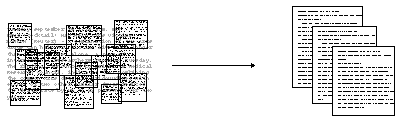
\includegraphics[scale=0.65]{ch2/assets/retrieve.png}
    \caption[InformationRetrival]{Visual representation of Information Retrieval\cite{gate2019}}
\label{fig:iret}
\end{figure}

\dots %TODO

The IR systems can be arranged in three groups based on its scale.
This groups are: Web search, personal information retrieval and institutional, and domain-specific search.

\section{Information Extraction}

As society became more data oriented having access to both structured and unstructured data became easy.
The difference between those those types of data is that structured data is semantically defined for a target domain and is interpreted with respect to category and context.
Therefor the need for applications capable of extracting structured data had increased.

Information Extraction (IE) is the name given to the process of automatically extracting structured information from an unstructured sources, mainly texts.

\begin{figure}[H]
\centering
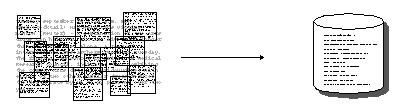
\includegraphics[scale=0.65]{ch2/assets/extract.png}
    \caption[InformationExtraction]{Visual representation of Information Extraction\cite{gate2019}}
\label{fig:iext}
\end{figure}

The result of an IE process is different for every case since it can be tailored according to the application needs.
Nowadays this applications can be used to fulfill personal, scientific and enterprise needs.

With the evolution of technology, IE also evolved and different techniques for the extraction of information were developed.
This techniques are the following: Rule-based, Statistical, Hybrids (both rule-based and statistical) and Conditional Random Fields\cite{sarawagi2008information}.

A rule-based approach was used by Del Gaudio et al.\cite{del2007automatic}.
In this paper the authors created a IE system that was capable extracting the definition of a word from texts written in Portuguese.

A statistical approach was used by Ventura\cite{ventura2014automatic}.
In his PhD report, he presented an alternative approach to the extraction of relevant terms from text.
Since relevance of a term is not conceptual, the author proposes to extract all concepts, which have a less fuzzy nature, and let the downstream application decide the relevance of those concepts.
A concept in the text mining area consists of a word or sequence of words which possess semantic value.

\subsection{Online Dictionaries}

One of the most known online dictionaries with \gls{LGP} content is the Spreadthesign\footnote{https://www.spreadthesign.com/}.
In this dictionary an user can search for a word and if there's a previously recorded video translation for that word, at the site database, it will be displayed for the user.
The search results only display the video of a person performing the corresponding sign, and the possibility to look at the same word in another sign language.

Another online dictionary that provides content for the \gls{LGP} users is the Infopédia\footnote{https://www.infopedia.pt/dicionarios/lingua-gestual}.
Although this is a Portuguese dictionary, it also contains a section for searching words in \gls{LGP}.
Here, the search results, not only provide a video translation of the word, but also an explanation in Portuguese on how to reproduce the sign shown in the video.

Online dictionaries as a solution, is limited by the database of prerecorded videos, and the \gls{LGP} lexicon.
The latter is a problem, because they focus on a direct translation, word to sign, instead of trying to translate the meaning of the word.

\subsection{Sign Language Interpreter}

In regard to the sign language interpreters in Portugal, there is CTILG\footnote{http://www.ctilg.pt/}, a company that provides professional \gls{LGP} translation services in workshops, classes, congresses, events and more.
This company is responsible for the live translation of some morning TV shows.

A more affordable solution for a regular \gls{LGP} user, is the Serviin\footnote{http://www.portaldocidadaosurdo.pt/Serviin} which is a service that provides an interpreter to work as a middle-man between a deaf person and a targeted service/company.
This solution is available as a mobile app, with a very low cost for the deaf user, or through a  web app that is free.

This solution is limited by the interpreters own knowledge and their cost.
Also by utilizing this solution, the \gls{LGP} user is sacrificing some of his autonomy.

\subsection{Readability Metrics}

Readability metrics are used to calculate a score\cite{meyer2003text}, that relates to the level of education a reader will need, to fully understand the context of a given text.
There are some widely known and used metrics for the English language, such as Flesh Reading Ease, New Dale-Chall, SMOG, Flesh-Kincaid, Gunning Fog and so on.

\dots %TODO

\subsection{Portuguese Readability Metrics}

In 2019, Antunes et al.\cite{antunes2019analyzing} published an article that adapted the values of the metrics used to calculate the readability of text in English so it could be applied to Portuguese.
The adapted readability metrics are presented in Table \ref{table:ptformulas}.

\begin{table}
    \caption{Adjusted Portuguese formulas.}
    \label{table:ptformulas}
    \begin{tabular}{l|l}
        \hline
        {} & {\bfseries Formula} \\
        \hline
        SMOG & \(16.830 \times \sqrt{CW \times 30 \div SE} - 23.809\)  \\
        \hline
        Flesch-Kincaid & \(0.883 \times WO \div SE + 17.347 \times SY \div WO - 41.239\) \\
        \hline
        ARI & \(6.286 \times CH \div WO + 0.927 \times WO \div SE - 36.551\) \\
        \hline
        Coleman Liau & \(5.730 \times CH \div WO - 171.365 \times SE \div WO - 6.662\) \\
        \hline
        Gunning Fog & \(0.760 \times WO \div SE + 58.600 \times CW \div WO - 12.166\) \\
        \hline
        \multicolumn{2}{l}{CH - characters, CW - complex words, SY - syllables, WO - words, SE - sentences}
    \end{tabular}
\end{table}

\section{Related Work}

After extensive research, this project seems to be the first to try to accomplish the goal of generating a definition to a given word or expression using Text Mining, Information Retrieval and Information Extraction.

Trying to achieve a similar goal using a different approach, Noraset Thanapon et al.\cite{noraset2016definition} chose a Deep Learning approach, that used a \gls{RNN} model that used distributed representations of words, also known as word embeddings, to generate dictionary representations.
The models were trained using a pre-defined data set.

Ni Ke et al.\cite{ni2017learning} also chose a Deep Learning approach and a \gls{RNN} model to generate a explanation of a given word or expression from "tweets" which is the name given to the posts made by the users of Twitter\footnote{https://twitter.com/}.
The focus was non-standard expressions, such as slang, presented in this posts.
The \gls{RNN} was trained using an online, user contributed, dictionary called Urban Dictionary\footnote{https://www.urbandictionary.com/}.

Giorgina Dinu et al.\cite{dinu2014make} tried to generate a phrase that best express the meaning contained in a distributional vector.
The test cases for this approach were a monolingual scenario where the phrase was generated in English and a cross-lingual setting where the vector was first used to generate the English expression and then translate it to Italian

Wiliam Dolan et al.\cite{dolan1993automatically} described an automated strategy to created a lexical knowledge base from online dictionaries.
This strategy was used to create a directed graph for semantic associations between words of the Longman Dictionary of Contemporary English\footnote{https://www.ldoceonline.com/}.
The authors argue that using a knowledge base provide a more detailed information about a word meaning than a standard lexical lookup.

Alan Akbik et al.\cite{akbik2009wanderlust} developed an algorithm called Wanderlust which automatically extracts semantic relations from natural language text.
This algorithm was applied to the English Wikipedia\footnote{https://en.wikipedia.org/} corpus and used to obtain semantic relations to populate a semantic wiki.

Atin Das et al.\cite{das2008neural} present a theoretical model based on using Neural Networks to extract what the authors calls 'featured words' from an article.
This 'featured words' are the words that best describe a given article.
Since this is a theoretical work there are no tests or specific use cases.

\section{Technology}

\dots

\subsection{NLTK}

\dots

\subsection{openNLP}

\dots

\subsection{Google Cloud NLP}

\dots

\subsection{Flask}

\dots

\subsection{React}

\dots

\subsection{Scrapy}

\dots

\subsection{Beautiful Soup 4 (bs4)}

\dots

\subsection{Virtual Sign Avatar}

The Virtual Sign Avatar\cite{escudeiro2015virtual} was a project developed by GILT (Games, Interaction and Learning Technologies) and is capable of translate Portuguese text to \gls{LGP}.

The visual part of the avatar as well as the animations it performs where created using Blender\footnote{https://www.blender.org/}.
Its appearance was designed to be as close as possible to the human body to help in the process of translation.

All the animations available to be performed by the avatar during the translation are stored in a database that relates each animation to the respective text.
When is requested the translation of a text that is not present in the database the avatar will perform the animation of each letter of that text.
